\documentclass[main.tex]{subfiles}

\begin{document}
    \section{Konzept}
    Die Webseite von CodeUp ist eine Plattform für Menschen, die sich für das Programmieren interessieren und ihre Fähigkeiten verbessern möchten.
    Der Hauptfokus liegt hierbei auf der Entwicklung einer ganzheitlichen Lernumgebung, die über das reine Lernen von Programmiersprachen und Konzepten hinausgeht und alle wichtigen Aspekte der Software-Entwicklung abdeckt.
    Dazu gehören unter anderem die Planung und Umsetzung von Projekten, die Zusammenarbeit mit anderen Entwicklern und die Veröffentlichung von eigenen Projekten.
    Da sich CodeUp vor allem an Schüler richtet, die noch keine oder nur wenig Erfahrung im Programmieren haben, wurden vor allem Unterrichtsrelevante Themen in den Vordergrund gestellt.
    Ebenfalls gibt es Integrationsmöglichkeiten für die Verwendung in der Schule oder in anderen Bildungsinstitutionen.
    Die Webseite ist so aufgebaut, dass sie sowohl für Anfänger als auch für Fortgeschrittene geeignet ist und eine Vielzahl von Funktionen bietet, die für beide Zielgruppen relevant sind.
    Auch die Wahl des Lernmediums ist wichtig, weshalb nach intensiver Recherche entschieden wurde, dass das Lernen über interaktive (Video-)Kurse am effektivsten ist.
    Diese interaktiven Kurse sind in verschiedene Lektionen unterteilt, die jeweils exakt einen Themenaspekt abdecken.


    \section{Technologie-Stack}
    CodeUp wurde mit modernen Web-Technologien entwickelt, um eine hohe Benutzerfreundlichkeit und Funktionalität zu gewährleisten.
    Da die Webseite aus vielen verschiedenen Komponenten besteht, wurde sie in einer Monorepo-Struktur organisiert.
    Für diese Monorepo-Struktur wurde das Werkzeug \dq Turborepo\dq\footnote{\bscite{turborepo}}\ verwendet, welches eine einfache Verwaltung von mehreren Paketen ermöglicht.
    Die Wahl der Programmiersprache fiel auf TypeScript, da diese eine statische Typisierung ermöglicht und so die Code-Qualität erhöht und die Fehleranfälligkeit reduziert.
    Im Kern besteht CodeUp aus einem Frontend- und einem Backend-Teil, die durch die Bibliothek \dq Next.js\dq\footnote{\bscite{nextjs}}\ miteinander verbunden sind.
    Allerdings wird nicht der von Next.js bereitgestellte HTTP-Server verwendet, sondern ein eigener, der auf dem Node.js-Modul \dq http\dq\ basiert.
    Für die Kommunikation zwischen Frontend und Backend wird eine REST-API verwendet, die über eine eigene Bibliothek abstrahiert wird (siehe~\ref{subsec:web_srv_communication}).
    Die Daten werden in einer MongoDB-Datenbank gespeichert, während Dateien in einem S3-kompatiblen Object-Storage abgelegt werden.
    Für die Benutzeroberfläche fiel die Wahl auf das Design-System \dq Chakra UI\dq\footnote{\bscite{chakraui}}, das eine Vielzahl an vorgefertigten Komponenten bietet und eine einfache Anpassung ermöglicht.
    Chakra UI wurde für CodeUp angepasst und um ein eigenes Theme erweitert, welches Farben, Schriftarten und andere Design-Elemente enthält.
    Die Webseite ist responsive gestaltet, sodass sie auf allen Geräten optimal dargestellt wird, was allerdings nicht in allen Bereichen (z.~B.~Code-Editoren) technisch möglich ist.
    Durch die Organisation in einer Git-Repository wird die Versionskontrolle gewährleistet und Fehler können frühzeitig erkannt und behoben werden.
    Notfalls kann auf ältere Versionen zurückgegriffen werden, um Fehler zu beheben.
    Bei der tatsächlichen Entwicklung wird auf JetBrains WebStorm\footnote{\bscite{webstorm}} als IDE gesetzt, da diese eine Vielzahl an Funktionen bietet und so produktives Arbeiten ermöglicht.


    \subsection{Sicherheit}
    Für die sichere Speicherung und spätere Validierung von Anmeldedaten wird das Password-Hashing-Verfahren sha256 verwendet.
    Dieses Verfahren bietet eine sogenannte Einwegverschlüsselung, sodass Klartext zwar in einen Hash umgewandelt werden kann, dieser aber nicht wieder in Klartext zurückverwandelt werden kann.
    Dies ist besonders wichtig, da die Sicherheit der Benutzerdaten oberste Priorität hat.
    Wenn ein Benutzer sich anmeldet, wird das eingegebene Passwort mit dem oben genannten Verfahren gehasht und mit dem in der Datenbank gespeicherten Hash verglichen.
    Sollten die beiden Hashes übereinstimmen, wird der Benutzer authentifiziert und erhält einen JWT (JSON Web Token)\footnote{\bscite{jwt}}, der für die weitere Kommunikation mit dem Server verwendet wird.
    Dieser JWT enthält Informationen über den Benutzer und wird bei jeder Anfrage an den Server mitgeschickt, um den Benutzer zu authentifizieren.
    Generell wird sämtlicher Datenverkehr über eine gesicherte HTTPS-Verbindung abgewickelt, um die Kommunikation zwischen Client und Server zu verschlüsseln.

    \subsection{Benutzeroberfläche und Design}
    Die Benutzeroberfläche wurde mit dem React.js\footnote{\bscite{react}} Framework entwickelt und besteht aus einer Vielzahl von Komponenten, die in einer Komponenten-Bibliothek organisiert sind.
    React ist eine Bibliothek, die es ermöglicht, Benutzeroberflächen aus wiederverwendbaren Komponenten zu erstellen und gleichzeitig eine interaktive Benutzererfahrung zu bieten.
    Um die Benutzerfreundlichkeit zu erhöhen, wurde die Webseite möglichst übersichtlich und intuitiv gestaltet.
    Das heißt konkret, dass alle wichtigen Funktionen leicht zugänglich sind und die Navigation so einfach wie möglich gestaltet wurde.
    Das Hauptmenü bildet hierbei den zentralen Anlaufpunkt für alle Funktionen und ist immer sichtbar, unabhängig von der Position auf der Webseite.
    Ebenfalls wurden mehrere Sprachen unterstützt, um die Webseite für eine größere Zielgruppe zugänglich zu machen.
    Diese Sprachen sind allerdings zum aktuellen Zeitpunkt nur für Text-basierte Inhalte verfügbar, da die Übersetzung von Videos und anderen dynamischen Inhalten zu aufwendig ist.
    Das Design der Webseite wurde so gewählt, dass es modern und ansprechend wirkt, aber gleichzeitig nicht zu überladen ist.
    Die Farbgebung ist dezent und aufeinander abgestimmt, um eine angenehme Benutzererfahrung zu gewährleisten.
    So wurde generell auf grelle Farben und zu viele Animationen verzichtet, um die Ablenkung des Benutzers zu minimieren.
    Die Farbkomposition besteht aus dunklen Grautönen für den Hintergrund und nicht wichtigen Elementen, während wichtige Elemente in einem hellen Gelb ({\color{cyellow}\texttt{\#F7DE1F}}) hervorgehoben werden.
    Es kommen allerdings selten auch andere Farben zum Einsatz, beispielsweise bei destruktiven Aktionen, die in einem kräftigen Rot ({\color{cred}\texttt{\#E03131}}) dargestellt werden.

    \subsection{Backend}
    Das Backend von CodeUp basiert auf dem Node.js-Framework und dem dazugehörigen \dq http\dq-Modul, welches die Erstellung eines HTTP-Servers ermöglicht.
    Neben dem HTTP-Server wird auch ein WebSocket-Server verwendet, um eine bidirektionale Kommunikation zwischen Client und Server zu ermöglichen.
    Für die WebSocket-Kommunikation wird die Bibliothek \dq socket.io\dq \footnote{\bscite{socketio}}\ verwendet.
    Die Datenspeicherung und spätere Verarbeitung erfolgt über eine MongoDB-Datenbank.
    MongoDB wurde initial in Betracht gezogen, da es eine Nicht-Relationale Datenbank ist und somit eine hohe Flexibilität bietet, die für CodeUp zwingend erforderlich ist.
    In dieser MongoDB-Datenbank werden sowohl die Benutzerdaten als auch sämtliche andere Daten der Platform gespeichert.
    Lediglich Dateien, die Benutzer hochladen oder durch das Anlegen von Projekten indirekt erstellen, werden separat im S3-kompatiblen Object-Storage MinIO gespeichert.
    MinIO ist eine Open-Source-Alternative zu Amazon S3 und ermöglicht die effiziente Speicherung von Dateien.

    \subsection{Kommunikation zwischen Frontend und Backend}\label{subsec:web_srv_communication}
    Die Kommunikation zwischen Frontend und Backend der Webseite erfolgt größtenteils über eine REST-API, also eine HTTP-Kommunikation zwischen dem Client und dem Server.
    Damit diese REST-API möglichst einfach in den Frontend-Code integriert werden kann, wurde eine separate Bibliothek entwickelt, die die Kommunikation abstrahiert und vereinfacht.
    Diese Bibliothek wird in allen Komponenten der Webseite verwendet und umfasst alle möglichen Funktionen und Endpunkte, die der Server bereitstellt.
    Benutzer können die CodeUp-REST-API auch in eigenen Projekten verwenden, weshalb die Bibliothek auch als eigenständiges Paket veröffentlicht wurde.
    Eine beispielhafte Nutzung der Bibliothek zur Authentifizierung eines Benutzers könnte wie folgt aussehen:
    \begin{lstlisting}[language=javascript]
import { REST } from "@codeupspace/rest";
REST.Account.loginWithUsername({
    username: "test",
    password: "test"
});
    \end{lstlisting}
    In diesem Beispiel wird ein Benutzer mit dem Benutzernamen \dq test\dq \ und dem Passwort \dq test\dq \ authentifiziert.
    Die REST-API-Bibliothek kümmert sich um die korrekte Kommunikation mit dem Server und gibt als Ergebnis immer ein Promise-Objekt des Typs \dq IResponse\dq\ zurück.
    Dies ist ein spezielles Interface, das aus einem Statuscode und einem Datenobjekt besteht:
    \begin{lstlisting}[language=javascript]
interface IResponse {
    status: number;
    payload: any;
}
    \end{lstlisting}
    Das Datenobjekt enthält die Antwort des Servers, die je nach Anfrage unterschiedlich sein kann.
    Der Statuscode gibt an, ob die Anfrage erfolgreich war oder nicht.

    \section{Funktionsumfang}
    \subsection{Generelle und globale Funktionen}
    \subsubsection{Anmelden}
    Bei der initialen Registrierung auf CodeUp hat der Benutzer die Möglichkeit, sich mit seiner E-Mail-Adresse und einem Passwort zu registrieren.
    Allerdings gibt es auch die Möglichkeit, sich mit GitHub, GitLab oder Discord anzumelden, sodass der Benutzer nicht extra ein Passwort erstellen muss.
    Nach der Registrierung wird eine E-Mail zur Bestätigung an die angegebene E-Mail-Adresse gesendet, um die Echtheit der Adresse zu überprüfen.
    Erst nach der Bestätigung kann der Benutzer sich anmelden und die Plattform nutzen.
    \subsubsection{Dashboard}
    Das Dashboard ist die zentrale Anlaufstelle für alle Benutzer und bietet eine Übersicht über alle wichtigen Informationen.
    Hier kriegt der Benutzer eine Übersicht über seine Kurse, Zertifikate, Aufgaben, Flussdiagramme, Snippets und Projekte.
    Ebenfalls gibt es die Möglichkeit, das Dashboard individuell anzupassen, indem der Benutzer die verschiedenen Sektionen verschieben oder ausblenden kann.
    Hierdurch wird der Benutzer aktiv in die Gestaltung seines Dashboards eingebunden und kann es so an seine Bedürfnisse anpassen.
    Das Dashboard ist so gestaltet, dass es auf allen Geräten optimal dargestellt wird und eine intuitive Bedienung ermöglicht.
    Des Weiteren gibt es auf dem Dashboard meist keine direkten Aktionen, sondern lediglich Links zu den entsprechenden Seiten, sodass der Benutzer nicht überfordert wird.
    \subsubsection{Einstellungen}
    Die Einstellungen-Seite bietet dem Benutzer die Möglichkeit, seine persönlichen Daten zu ändern.
    Dabei kann er seine E-Mail-Adresse, sein Passwort und seinen Vor- und Nachnamen verändern.
    Eine Änderung des Benutzernamens ist nicht möglich, da dieser teilweise als eindeutiger Identifikator verwendet wird.
    Neben den persönlichen Daten kann der Benutzer auch die Zwei-Faktor-Authentifizierung aktivieren, um sein Konto zusätzlich zu schützen.
    Hierbei wird ein QR-Code angezeigt, den der Benutzer mit einer Authenticator-App scannen kann, um den Zwei-Faktor-Authentifizierungs-Code zu erhalten.
    Sollte die Zwei-Faktor-Authentifizierung aktiviert sein, wird der Benutzer bei jedem Anmeldevorgang nach dem Code gefragt.
    Zum Deaktivieren der Zwei-Faktor-Authentifizierung muss der Benutzer ebenfalls den Code aus seiner Authenticator-App eingeben.
    Auch das Löschen des Kontos ist möglich, allerdings gibt es hier mehrere Kontrollmechanismen, um sicherzustellen, dass der Benutzer das Konto und alle damit verbundenen Daten wirklich löschen möchte.
    \subsubsection{Spracheinstellungen}
    Der Benutzer hat die Möglichkeit, die Sprache der Webseite zu ändern.
    Dies funktioniert über die Schaltfläche im Fußzeilenbereich, die die aktuell ausgewählte Sprache in Form einer Flagge anzeigt.
    Durch Klicken auf die Schaltfläche öffnet sich ein Dropdown-Menü, in dem der Benutzer die gewünschte Sprache auswählen kann.
    Aktuell werden Deutsch und Englisch manuell übersetzt, wobei Deutsch als Standardsprache festgelegt ist.
    Automatische Übersetzungen gibt es für Französisch, Spanisch, Italienisch, Niederländisch, Polnisch und Portugiesisch.
    Diese automatischen Übersetzungen basieren auf der LibreTranslate-API\footnote{\bscite{libretranslate}}, die eine einfache und zuverlässige Übersetzung ermöglicht.
    Sprachen, die automatisch übersetzt werden, bieten keine perfekte Übersetzung, sind aber in den meisten Fällen verständlich und ermöglichen es dem Benutzer, die Webseite in seiner Muttersprache zu nutzen.
    Aktuell ist es nicht möglich, Videos in einer anderen Sprache anzusehen, da die Übersetzung von Videos zu teuer und aufwendig ist.
    \subsubsection{Level-System}
    Das Level-System ist eine Art Belohnungssystem, das den Benutzer für seine Aktivitäten auf der Plattform belohnt.
    Viele Aktionen, wie das Erstellen von Projekten, das Abschließen von Zertifikaten oder das Lösen von Challenges, geben dem Benutzer Erfahrungspunkte, die ihn im Level aufsteigen lassen.
    Hierdurch wird der Benutzer dazu motiviert, sich aktiv auf der Plattform zu beteiligen und seine Fähigkeiten zu verbessern.
    Jedes Level benötigt eine bestimmte Anzahl von Erfahrungspunkten, um erreicht zu werden.
    Diese Anzahl steigt mit jedem Level, sodass es immer schwieriger wird, ein neues Level zu erreichen.
    Hierzu wird eine einfache Formel verwendet, die die Anzahl der benötigten Erfahrungspunkte berechnet:
    \begin{equation}
        \text{Level} = \text{Erfahrungspunkte}^{\frac{1}{3}}
    \end{equation}
    \subsubsection{Admin-Panel}
    Das Admin-Panel ist eine spezielle Seite, die nur für Administratoren zugänglich ist und es ihnen ermöglicht, die Plattform zu verwalten.
    Hier können Administratoren Benutzer sperren, Projekte löschen, Kurse überprüfen und andere administrative Aufgaben erledigen.
    Das Admin-Panel ist so gestaltet, dass es einfach zu bedienen ist und alle wichtigen Funktionen auf einen Blick bietet.
    Des Weiteren bietet das Admin-Panel eine Übersicht über Statistiken, wie die Anzahl der Benutzer, die Anzahl der Kurse und die Anzahl der Projekte.
    Neben den globalen Analysen gibt es auch die Möglichkeit detaillierte Analysen für einzelne Benutzer durchzuführen.
    Diese Analyse beinhaltet Informationen über die Aktivitäten des Benutzers, wie die Anzahl der Aufrufe und welche Seiten aufgerufen wurden.
    Zu Verbesserungszwecken und um Fehler schneller zu identifizieren wurde ein Session-Recording-Werkzeug namens rrweb\footnote{\bscite{rrweb}} integriert.
    Hierdurch können Administratoren die Aktionen jedes einzelnen Aufrufs nachvollziehen und so Fehler schneller identifizieren.
    rrweb ist so gestaltet, dass keine sensiblen Daten aufgezeichnet werden und die Privatsphäre der Benutzer gewahrt bleibt.
    Durch das Admin-Panel können viele verschiedene Facetten der Plattform verwaltet werden, hierzu zählen:
    \begin{itemize}
        \item Benutzer: Hier können Benutzer gesperrt, gelöscht oder bearbeitet werden.
        Im Notfall kann sich ein Administrator auch als Benutzer einloggen, um Probleme zu lösen.
        \item Blog: Administratoren können Blog-Beiträge erstellen, bearbeiten und löschen.
        \item CDN: Das Content-Delivery-Network kann über das Admin-Panel konfiguriert und verwaltet werden.
        Hier können global verfügbare Dateien, wie Bilder und Videos, hochgeladen und verwaltet werden.
        \item Challenges: Administratoren können Challenges erstellen, bearbeiten und löschen.
        \item Code-Snippets: Code-Snippets von Benutzern können in dieser Ansicht verwaltet werden.
        \item Discovery: Hier können Discovery-Einträge notfalls manuell gelöscht werden, falls sie gegen die Richtlinien verstoßen.
        \item Editor: Verwaltung der Projekte, die mit dem Editor (v2) erstellt wurden.
        \item Fehler: Hier werden alle Fehler und Warnungen aufgelistet, die auf der Plattform aufgetreten sind.
        \item Flows: Administratoren können Flussdiagramme von Benutzern einsehen, bearbeiten und löschen.
        \item IDE: Verwaltung der Projekte, die mit dem IDE (v1) erstellt wurden.
        \item Kids: Verwaltung der CodeUp-Kids-Projekte.
        \item Meinungen: Berechtigte Benutzer können in dieser Ansicht Meinungen über die Plattform verwalten, die auf der Homepage angezeigt werden.
        \item Organisationen: Hier können Organisationen erstellt, bearbeitet und gelöscht werden.
        \item Profile: Verwaltung der Benutzerprofile, inklusive der Möglichkeit, Benutzer zu sperren oder zu löschen.
        Mit Profilen sind hier Profile aus dem Forum gemeint, nicht die tatsächlichen Benutzerkonten.
        \item Projektideen: Administratoren können Projektideen erstellen, bearbeiten und löschen.
        \item Replay: Zentrale Anlaufstelle für das Session-Recording-Tool rrweb.
        \item Shorts: Verwaltung von gekürzten URLs, die auf andere Webseiten verweisen.
        Diese sind nur für Administratoren sichtbar und können nicht von Benutzern erstellt werden.
        \item To-do: Hier können Administratoren To-do-Listen von Benutzern verwalten.
        \item Zertifikate: Verwaltung der Zertifikate, die Benutzer erhalten, wenn sie einen Kurs erfolgreich abgeschlossen haben.
    \end{itemize}
    Das Admin-Panel ist nicht zu jeder Zeit auf den Funktionsumfang der Plattform angepasst, sondern wird regelmäßig aktualisiert und erweitert.
    Dies hat zur Folge, dass teilweise manuelle Eingriffe in die Datenbank notwendig sind, um bestimmte Funktionen zu ermöglichen.
    In der Abbildung~\ref{fig:admin-panel} sind die Hauptfunktionen des Admin-Panels dargestellt.
    \begin{figure}[h]
        \centering
        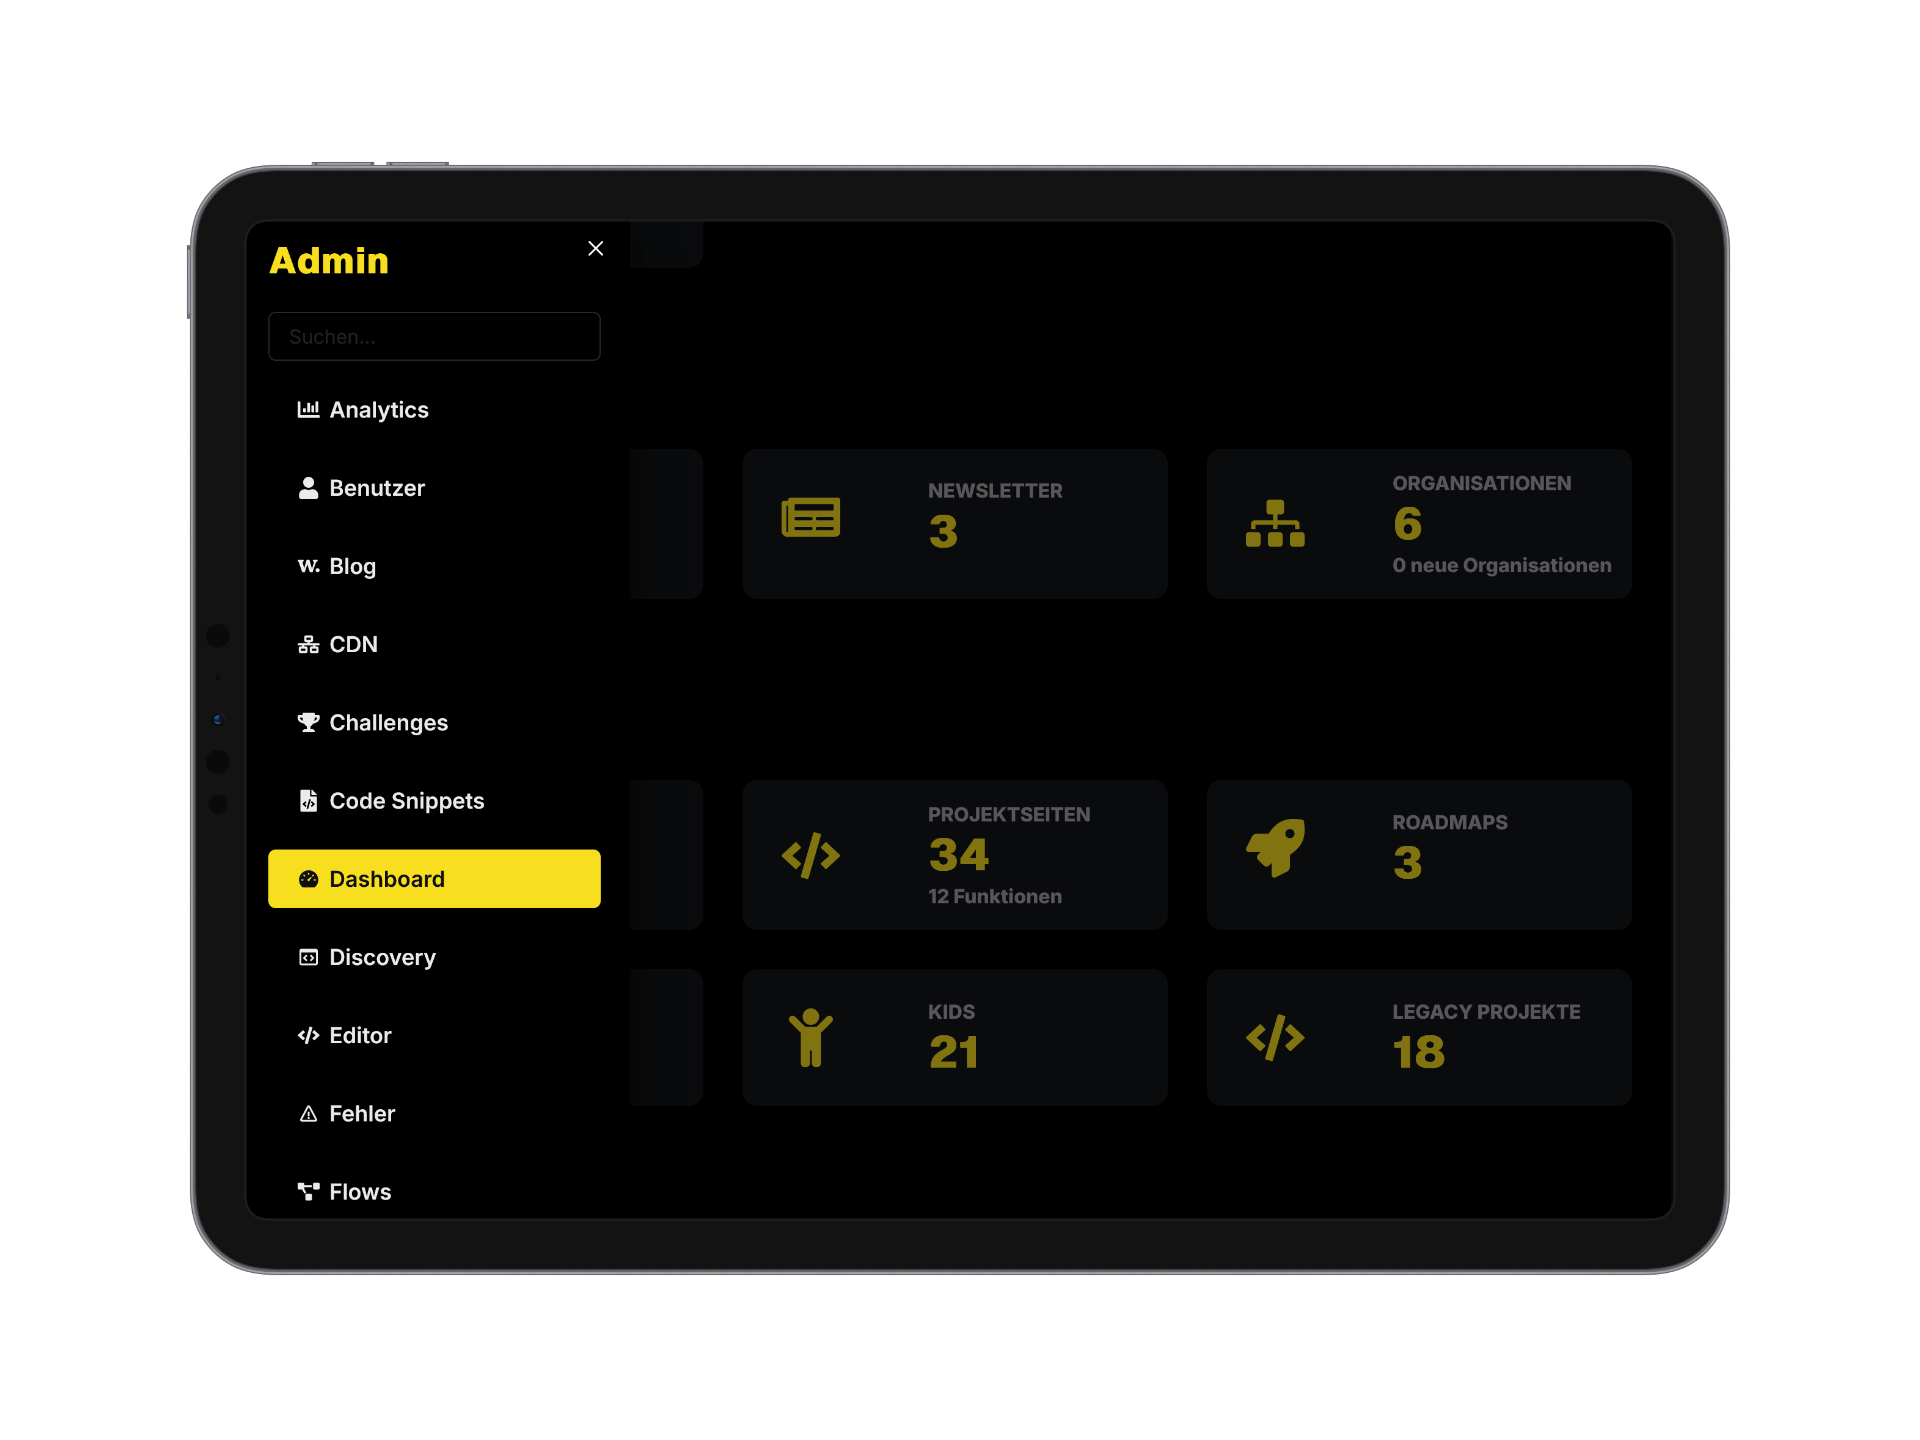
\includegraphics[width=0.5\textwidth]{assets/admin-panel}
        \caption{Admin-Panel}
        \label{fig:admin-panel}
    \end{figure}
    \subsubsection{Organisationen}
    Organisationen sind eine Möglichkeit für Bildungseinrichtungen, Unternehmen oder andere Gruppen, ihre Mitglieder zu organisieren und ihnen spezielle Funktionen zur Verfügung zu stellen.
    Jede Organisation hat einen Gründer, der automatisch Administrator ist und weitere Mitglieder hinzufügen kann.
    Organisationen haben die Möglichkeit, eigene Kurse zu erstellen und diese allen Mitgliedern zur Verfügung zu stellen.
    Ebenfalls können Mitteilungen an alle Mitglieder verschickt werden, um wichtige Informationen zu verbreiten.
    \subsubsection{Creator Studio}
    Das Creator Studio ist der zentrale Anlaufpunkt für alle Benutzer, die eigene Kurse erstellen möchten.
    Hier können Benutzer neue Kurse erstellen und bestehende Kurse bearbeiten.
    Das Veröffentlichen der Kurse erfolgt nach der Überprüfung durch das CodeUp-Team, um die Qualität der Kurse zu gewährleisten.
    Grundsätzlich gibt es drei Sichtbarkeitsstufen für Kurse:
    \begin{itemize}
        \item \textbf{Privat}: Der Kurs ist nur für den Ersteller sichtbar und kann nicht von anderen Benutzern genutzt werden.
        \item \textbf{Öffentlich}: Der Kurs ist für alle Benutzer sichtbar und kann von jedem angesehen werden.
        \item \textbf{Organisation}: Der Kurs ist für alle Benutzer einer bestimmten Organisation sichtbar und kann nur von diesen angesehen werden.
        Der Kurs-Ersteller kann bestimmen, welche Organisation Zugriff auf den Kurs hat, muss dafür allerdings auch Gründer oder Administrator dieser Organisation sein.
    \end{itemize}
    Ein Creator kann für jeden seiner Kurse ein individuelles Vorschaubild festlegen und eine Beschreibung hinzufügen, um den Kurs attraktiver zu gestalten.
    Ebenfalls kann der Creator die Reihenfolge der Lektionen festlegen und so den Lernprozess steuern.
    Die Änderung und Erstellung von Lektionen erfolgt über ein Drag-And-Drop Menü, das das neue Anordnen der Lektionen ermöglicht.
    Auch das Erstellen eines Zertifikats wird über das Create Studio abgewickelt, wobei der Creator die Fragen und Antworten festlegen kann.
    Die Fragen können entweder Multiple-Choice, Code-Vervollständigung, Code-Vergleich oder Code-Überprüfung sein.
    Ebenfalls kann der Creator festlegen, wie viele Fragen richtig beantwortet werden müssen, um das Zertifikat zu erhalten.
    Das funktioniert ebenfalls über eine Drag-And-Drop Oberfläche, die auch noch spätere Änderungen an der Reihenfolge zulässt.
    Wenn der Creator einen Kurs erstellt, muss er angeben, ob dieser ein Video- oder ein interaktiver Kurs ist.
    Bei interaktiven Kursen kann der Creator die Übungen festlegen, die der Benutzer lösen muss, um die Lektion abzuschließen.
    Bei Videokursen kann der Creator die Videos hochladen und eine Beschreibung hinzufügen.
    Wenn eine Video-Lektion eingefügt wird, muss ein Quiz hinzugefügt werden, das aus mindestens einer Frage besteht.
    Es ist ebenfalls möglich, die Lektionstypen zu mischen, sodass ein Kurs sowohl aus Video- als auch aus interaktiven Lektionen bestehen kann.
    Allerdings muss der Kurs eine bevorzugte Art haben, die bei der Erstellung festgelegt wird und nicht mehr geändert werden kann.
    In Abbildung~\ref{fig:creator-studio} sind die Hauptfunktionen des Creator Studios dargestellt.
    \begin{figure}[h] % options: h, t, b, p
        \centering
        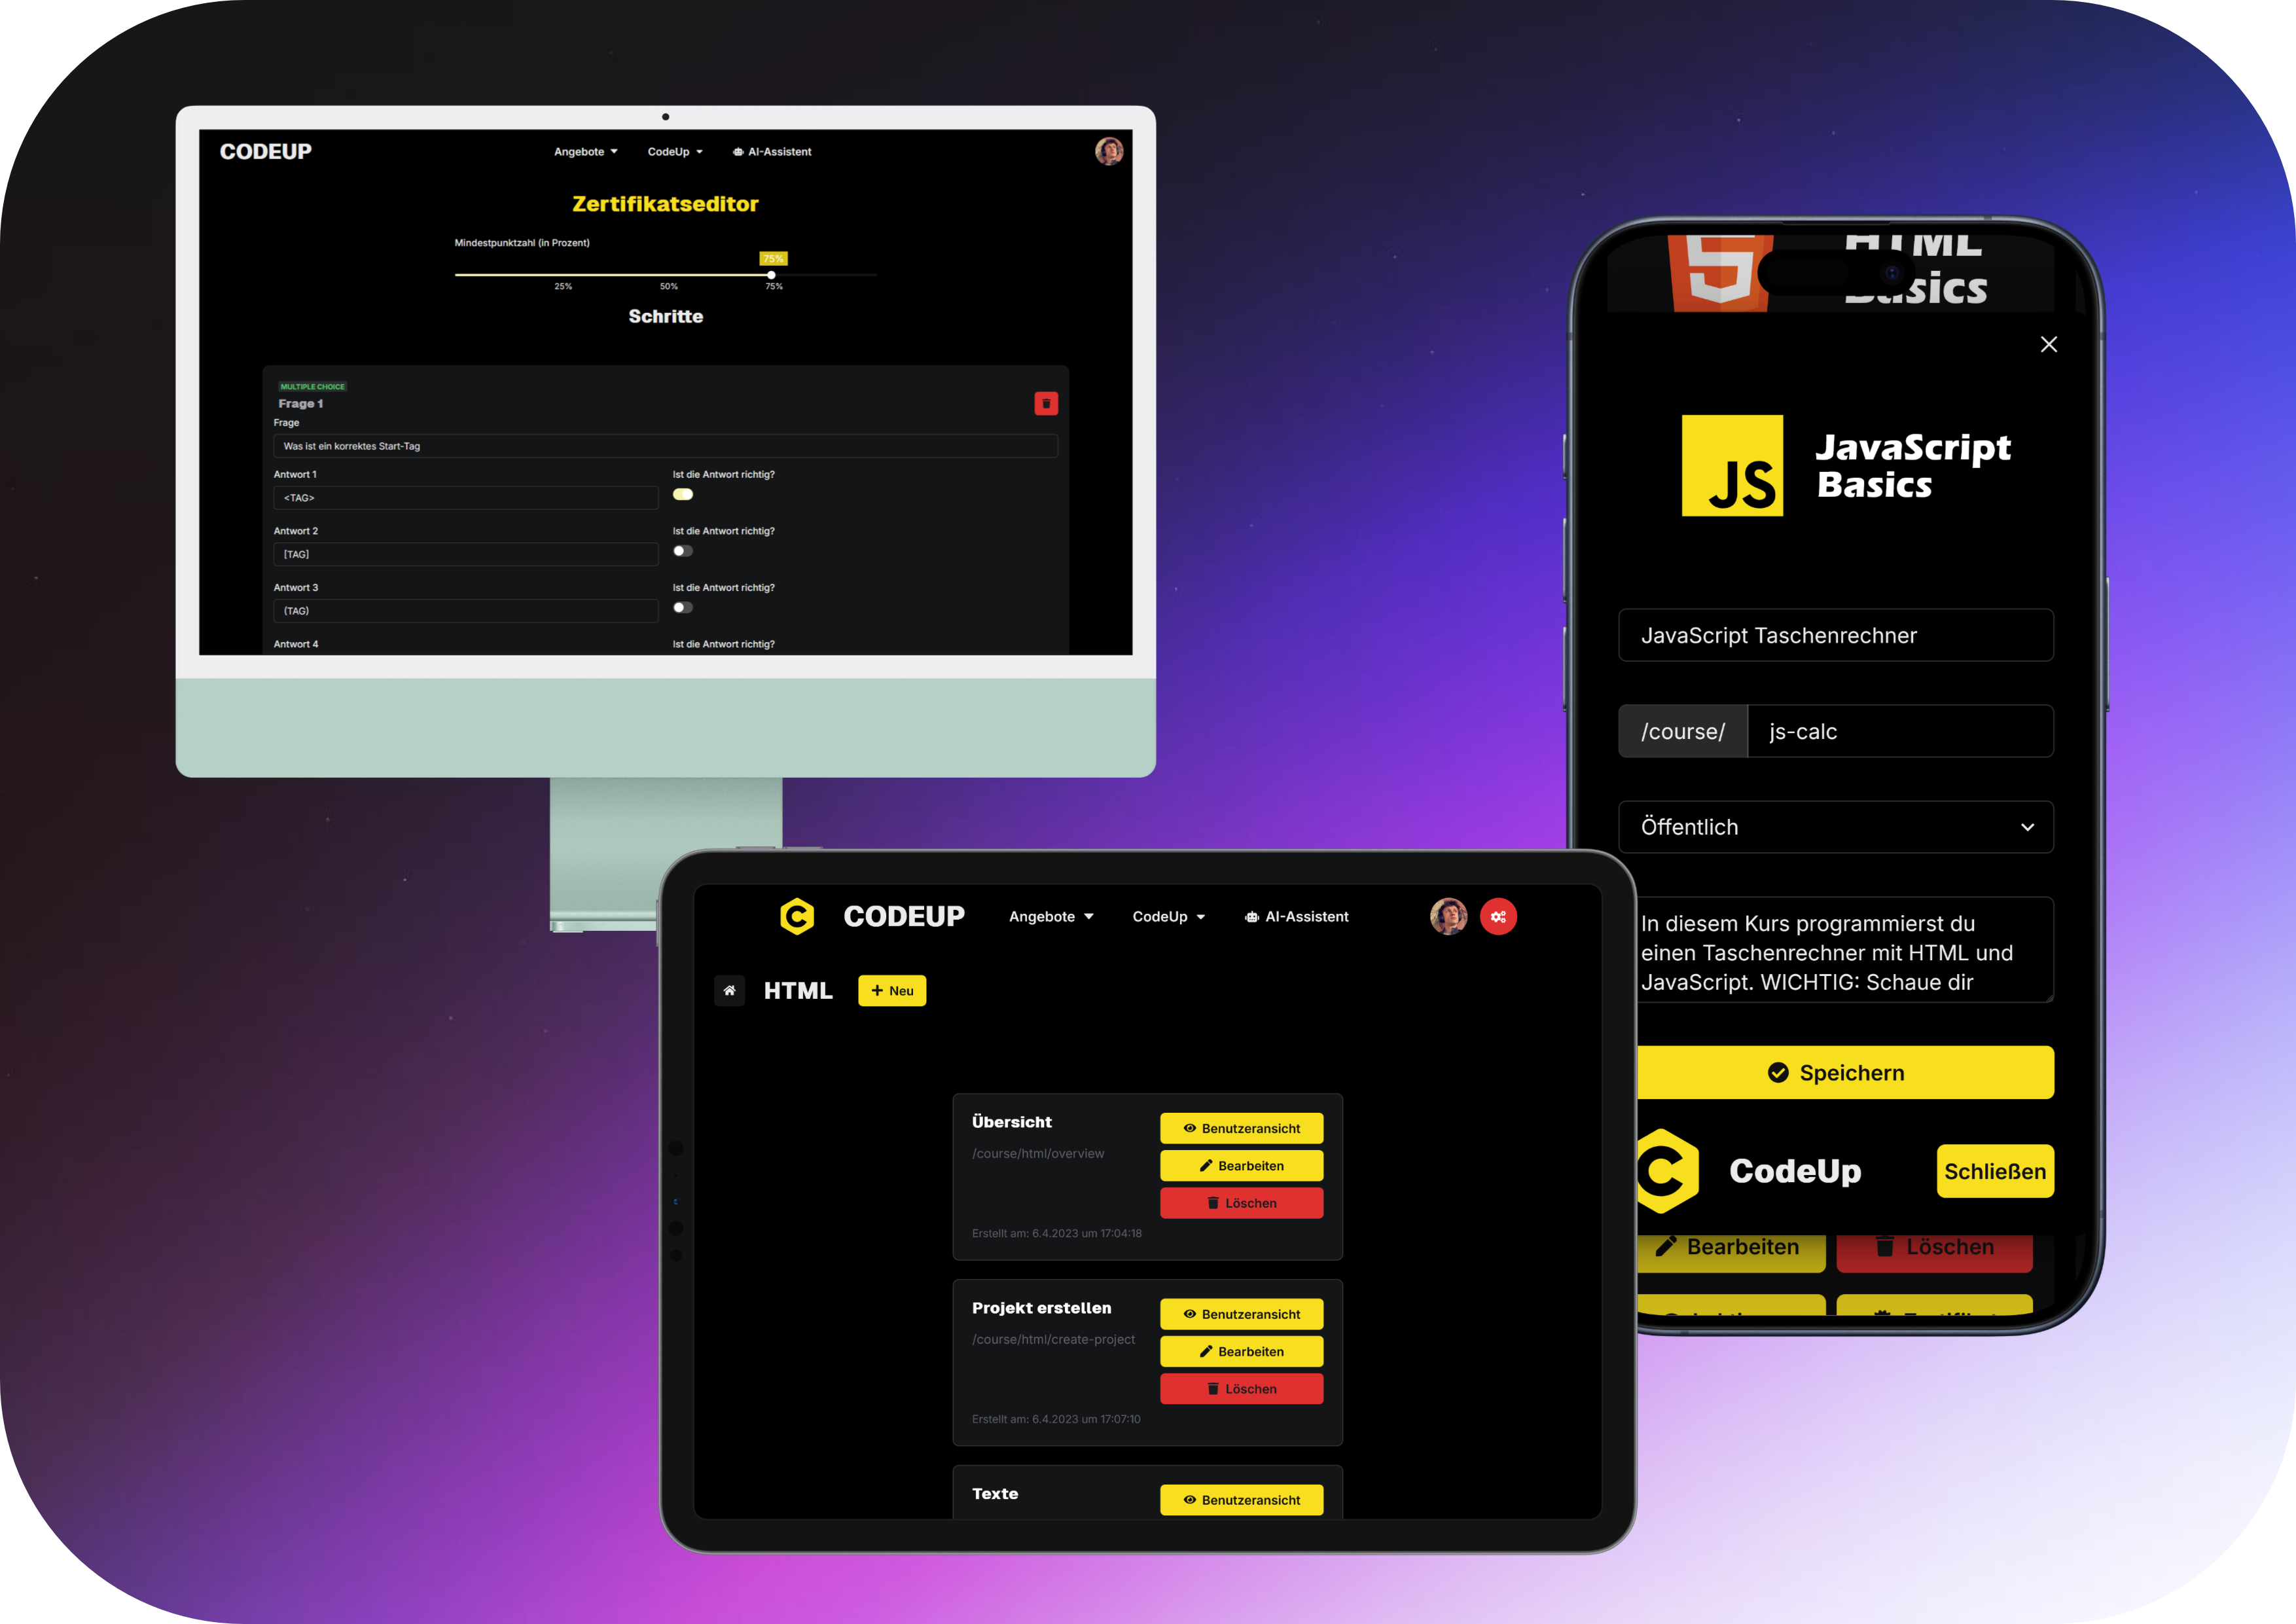
\includegraphics[width=0.6\textwidth]{assets/creator-studio}
        \caption{Creator Studio}
        \label{fig:creator-studio}
    \end{figure}
    \subsubsection{KI-Assistent}
    Der KI-Assistent ist ein Feature, das dem Benutzer individuelle Hilfe und Unterstützung bietet.
    Er kann Fragen beantworten, Tipps geben und den Benutzer bei der Lösung von Problemen unterstützen.
    Der KI-Assistent ist in der Lage, den Code des Benutzers zu analysieren und ihm Vorschläge zu machen, wie er diesen verbessern kann.
    Das ganze System basiert auf dem OpenAI-Modell GPT-4o-mini\footnote{\bscite{gpt4o-mini}}, das speziell für die Verwendung in Chatbots und anderen KI-Systemen entwickelt wurde.
    Aufgebaut ist der KI-Assistent in einer Chat-Oberfläche, die es dem Benutzer ermöglicht, direkt mit ihm zu interagieren und auf ältere Konversationen zugreifen zu können.
    \subsection{Lernen}
    \subsubsection{Kurse}
    CodeUp bietet eine Vielzahl an Kursen an, von denen jeder einzelne ein spezifisches Thema, wie beispielsweise eine Programmiersprache oder ein Konzept, abdeckt.
    Grundsätzlich besteht jeder Kurs aus mehreren Lektionen, die jeweils einen Teilaspekt des Themas behandeln.
    Es gibt zwei verschiedene Arten von Kursen:
    \begin{itemize}
        \item \textbf{Interaktive Kurse}: Diese Kurse sind Text-basiert und bieten interaktive Übungen an, die den Benutzer dazu auffordern, selber Code zu schreiben.
        Hierbei beginnt jede Lektion mit einem kurzen Text, der das Thema einführt, gefolgt von einer oder mehreren Übungen, die den Benutzer dazu auffordern, Code zu schreiben.
        Jede Übung ist von einem Beispiel begleitet, das dem Benutzer zeigt, wie die Lösung aussehen könnte.
        \item \textbf{Videokurse}: Diese Kurse bestehen aus einer Reihe von Videos.
        Hierbei gibt es nach jedem Video ein Quiz, das den Benutzer dazu ermutigt, sein Wissen zu testen und ggf. die Lektion zu wiederholen.
    \end{itemize}
    Die Video-Lektionen sind in der Regel kurze Videos (ca.~5-10 Minuten) und behandeln ein spezifisches Thema.
    Interaktive Lektionen bestehen meist aus 5--10 Übungen und enthalten aktuell kein Quiz, da das Wissen durch das Schreiben von Code getestet wird.
    Videos werden auf der Video-Plattform YouTube gehostet und in die Webseite eingebettet, während interaktive Kurse direkt auf der Webseite gehostet werden.
    Durch die Auslagerung auf YouTube können die Kosten für die Infrastruktur reduziert werden, da YouTube die Videos kostenlos bereitstellt.
    \subsubsection{Challenges}
    Challenges sind kleine Programmieraufgaben, die der Benutzer lösen muss.
    Diese Aufgaben können in JavaScript, TypeScript, Python, Go und Java gelöst werden und decken verschiedene Schwierigkeitsgrade ab.
    Jede Challenge besteht aus einer Beschreibung, die das Problem erklärt, und einem Code-Editor, in dem der Benutzer seine Lösung schreiben kann.
    Nachdem der Benutzer seine Lösung eingereicht hat, wird diese automatisch getestet und das Ergebnis angezeigt.
    Der Benutzer kann seine Lösung so oft ändern, wie er möchte, bis er mit dem Ergebnis zufrieden ist.
    Auch das erneute Übermitteln der Lösung ist möglich, um das Ergebnis zu aktualisieren.
    Technisch gesehen wird der eingegebene Code in einem isolierten Docker-Container ausgeführt, um die Sicherheit der Plattform zu gewährleisten.
    In Zukunft ist geplant, Challenges auch in anderen Programmiersprachen anzubieten und die Ausführung des Codes auf eine externe Plattform auszulagern, um die Sicherheit weiter zu erhöhen.
    \subsubsection{Zertifikate}
    Benutzer haben die Möglichkeit für absolvierte Kurse ein Zertifikat zu erlangen, um anderen ihre Fähigkeiten zu zeigen.
    Diese Zertifikate werden nicht automatisch vergeben, sondern müssen durch einen Test erworben werden.
    Diese Tests bestehen aus einer Reihe von Fragen, die das Wissen des Benutzers über das Thema des Kurses testen.
    Es gibt vier verschiedene Arten von Fragen:
    \begin{itemize}
        \item \textbf{Multiple-Choice}: Der Benutzer muss eine von mehreren vorgegebenen Antworten auswählen.
        \item \textbf{Code vervollständigen}: Der Benutzer muss fehlende Teile eines Code-Snippets ergänzen.
        \item \textbf{Code Vergleich}: Der Benutzer bekommt eine Ausgabe und muss aus zwei Codes denjenigen auswählen, der diese Ausgabe erzeugen.
        \item \textbf{Code Überprüfung}: Der Benutzer muss angeben, ob der Code Fehler enthält oder nicht.
    \end{itemize}
    Jedes Zertifikat hat einen individuellen Schwellenwert, der erreicht werden muss, um das Zertifikat zu erhalten.
    Dieser liegt standardmäßig bei 75\%, kann aber von den Kurs-Erstellern individuell angepasst werden.
    \subsection{Austauschen}
    \subsubsection{Forum}
    Durch das Forum können sich Benutzer untereinander austauschen und Fragen stellen.
    Hierbei gibt es die Möglichkeit, Text-Beiträge zu erstellen, die von anderen Benutzern kommentiert und mit einem Herz markiert werden können.
    Allerdings ist es ebenfalls möglich, Beiträge zu erstellen, die Bilder oder andere Medien, wie Dateien enthalten.
    Um dies zu ermöglichen, wird nach der Erstellung eines Beitrags im Hintergrund dieser analysiert und ggf. ein sogenanntes \dq Embed\dq\ erstellt.
    Diese \dq Embeds\dq\ sind spezielle Anhänge an einen Beitrag, die von der Webseite erkannt und entsprechend dargestellt werden.
    Datei-Uploads sind grundsätzlich erlaubt, allerdings gibt es eine maximale Dateigröße von 2~MB, um die Serverlast zu reduzieren, da die Dateien direkt in der Infrastruktur von CodeUp gespeichert werden.
    Neben den Beiträgen kann ein Benutzer auch ein eigenes Profil erstellen.
    Auf diesem Profil kann er eine Webseite verlinken, dies könnte zum Beispiel ein Projekt sein, das mit CodeUp veröffentlicht wurde.
    Neben der Einbindung einer Webseite kann der Benutzer außerdem seinen Wohnort und seinen Geburtstag eintragen.
    Diese Informationen sind allerdings, genauso wie eine Beschreibung, optional und müssen nicht ausgefüllt werden.
    Damit andere Benutzer besser einschätzen können, wenn sie um Hilfe bitten, gibt es die Möglichkeit, erworbene Zertifikate auf dem Profil anzuzeigen.
    Auch hier hat der Profilbesitzer die freie Wahl, welche Zertifikate angezeigt werden und welche nicht.
    Um eine direktere und private Kommunikation zu ermöglichen, gibt es eine Chat-Funktion, die mittels WebSockets in Echtzeit funktioniert.
    Hierdurch können Benutzer sich gegenseitig bestmöglich unterstützen und Fragen können schneller beantwortet werden.
    \subsubsection{Discovery}
    Das Discovery-Feature ermöglicht es Benutzern, eigene Projekte zu veröffentlichen und anderen Benutzern zur Verfügung zu stellen.
    Auch das Suchen und Entdecken von Projekten anderer Benutzer ist möglich, um sich inspirieren zu lassen oder von anderen zu lernen.
    Man kann Projekte mit einer Sternen-Bewertung von eins bis fünf versehen, um anderen eine Einschätzung über die Qualität des Projekts zu geben.
    Ebenfalls gibt es die Möglichkeit, Projekte zu kommentieren und Fragen zu stellen, um mehr über das Projekt zu erfahren.
    \subsection{Planen}
    \subsubsection{Aufgaben-Planung}
    Die Aufgaben-Planung soll Benutzern die Möglichkeit geben, ihre Projekte zu planen und zu strukturieren.
    Hierbei wird auf eine einfache To-do-Liste gesetzt, die es dem Benutzer ermöglicht, Aufgaben zu erstellen und zu verwalten.
    Jede Aufgabe besteht aus einem Titel, einer Beschreibung und einem Status, der angibt, ob die Aufgabe abgeschlossen ist oder nicht.
    Der Benutzer kann Aufgaben erstellen, bearbeiten und löschen, um seinen Arbeitsablauf zu organisieren.
    Diese To-do-Listen sollen dem Benutzer helfen, den Überblick über seine Projekte zu behalten, indem er große Aufgaben in kleinere Teilaufgaben unterteilt.
    \subsubsection{Flußdiagramme}
    Flussdiagramme sind ein wichtiges Werkzeug, um den Ablauf von Programmen zu visualisieren und zu planen.
    In CodeUp können sie dazu genutzt werden den Ablauf von konkreten Funktionen, wie einer Schaltfläche oder einer Animation, zu planen.
    Um eine möglichst einfache und intuitive Bedienung zu gewährleisten, wurde auf komplexe Verzweigungen und Schleifen verzichtet.
    Damit der Benutzer sein Flussdiagramm personalisieren kann, gibt es die Möglichkeit, Knoten zu färben und Kanten zu animieren oder mit einem Text zu versehen.
    \subsection{Entwickeln}
    Der Entwicklungsbereich von CodeUp ist der Bereich, der die meisten Änderungen und Erweiterungen erfahren hat.
    Es gibt mehrere verschiedene Editoren, die im Laufe der Zeit entwickelt wurden und jeweils unterschiedliche Funktionen bietet.
    Dabei ist die Dev-Suite der neuste Editor und bietet die meisten Funktionen, während der Editor (v2) und der IDE (v1) eher für spezielle Anwendungsfälle gedacht sind.
    \subsubsection{IDE (v1)}
    Die IDE (v1) ist ein einfacher Code-Editor, der es dem Benutzer ermöglicht, Code zu schreiben und auszuführen.
    Hierbei ist ausschließlich Frontend-Webentwicklung möglich, da der Code direkt im Browser des Benutzers ausgeführt wird.
    Der Editor bietet Syntax-Hervorhebung, Autovervollständigung und eine Vorschau-Funktion, um dem Benutzer ein möglichst angenehmes Arbeiten zu ermöglichen.
    Ebenfalls gibt es die Möglichkeit, Dateien zu speichern und zu laden, um den Code auch später noch bearbeiten zu können.
    Aufgebaut ist der Editor in Projekten, die aus mehreren Dateien bestehen können.
    Der Benutzer ist selbst für die Organisation der Dateien verantwortlich, da der Editor keine spezielle Struktur vorgibt.
    Dies beinhaltet auch das Verbinden von Dateien, um beispielsweise eine CSS-Datei in eine HTML-Datei einzubinden.
    \subsubsection{Editor (v2)}
    Der Editor (v2) ist ein fortgeschrittener Code-Editor, der es dem Benutzer ermöglicht, Back- und Frontend-Webentwicklung zu betreiben.
    Hierbei ist der Editor ebenfalls in Projekte organisiert, die allerdings nicht im klassischen Sinne aus mehreren Dateien bestehen.
    Viel mehr besteht ein Projekt aus mehreren Seiten, die jeweils HTML oder InCode als Grundgerüst haben und optional durch Resourcen, wie CSS- oder JavaScript-Dateien, erweitert werden können.
    Des Weiteren gibt es neben den Seiten auch sogenannte Serverless-Funktionen, die es dem Benutzer ermöglichen, einfache Server-Logik zu schreiben.
    Diese Funktionen werden auf einem Server als isolierte Docker-Container ausgeführt und können von den Seiten aufgerufen werden.
    Durch die Isolierung in einem Docker-Container kann es zu größeren Wartezeiten kommen, da der Container erst gestartet werden muss.
    Jede Funktion hat eine maximale Laufzeit von 10 Sekunden, um die Serverlast zu reduzieren und Funktionen vorzubeugen, die beispielweise als Crypto-miner missbraucht werden könnten.
    Der Editor (v2) bietet ebenfalls Syntax-Hervorhebung, Autovervollständigung und eine Vorschau-Funktion, um dem Benutzer ein möglichst angenehmes Arbeiten zu ermöglichen.
    Um eine schnellere Entwicklung zu ermöglichen, ist der Editor komplett auf WebSockets aufgebaut, sodass der Benutzer Änderungen in Echtzeit sehen kann.
    Durch die Verwendung von WebSockets wird eine kollaborative Entwicklung ermöglicht, da mehrere Benutzer gleichzeitig an einem Projekt arbeiten können und die Änderungen andere direkt sehen können.
    Dabei können maximal 10 Benutzer gleichzeitig an einem Projekt arbeiten, da es ansonsten zu Performance-Problemen kommen könnte.
    Der Ersteller des Projektes kann über den Mitwirkenden-Dialog Benutzer hinzufügen oder entfernen und deren Rechte festlegen.
    Auch ein Export des Projektes ist möglich, um es lokal zu speichern.
    Für das Hosting auf einem anderen Server außerhalb der CodeUp Umgebung ist ein Export zwar möglich, erfordert aber eine Anpassung des Codes, da das Format der Dateien speziell auf CodeUp zugeschnitten ist und keine allgemein gültige Struktur bietet.
    Durch die Integration der statischen Dateien können Benutzer beliebige Dateien, wie Bilder oder Videos, hochladen und in ihr Projekt einbinden.
    Diese Dateien können über eine URL aufgerufen werden, die auf den CodeUp-Server verweist.
    Durch die Abstraktion der Dateien bietet sich dieser Editor besonders für Anfänger an, die schnell und einfach Webseiten erstellen möchten.
    Anfänger können sich so nämlich auf die eigentliche Programmierung konzentrieren und müssen sich nicht um die Verlinkung oder Organisation der Dateien kümmern.
    \subsubsection{Dev-Suite (v3)}
    Die Dev-Suite (v3) ist der neuste und fortschrittlichste Editor, der in CodeUp enthalten ist.
    Er bietet die meisten Funktionen und ist speziell für fortgeschrittene Benutzer gedacht, die eine umfangreiche Entwicklungsumgebung benötigen.
    Wie die anderen Editoren ist auch die Dev-Suite in Projekte organisiert.
    Diese bestehen aber, wie bei der IDE (v1), aus mehreren Dateien, die der Benutzer selbst organisieren muss.
    Die Besonderheit ist, dass die Dev-Suite alle Aspekte der Entwicklung abdeckt, von der Planung über die Dokumentation, bis hin zur Entwicklung und der schlussendlichen Veröffentlichung.
    Es werden viele verschiedene Aspekte der CodeUp Webseite in der Dev-Suite abgedeckt, wie beispielsweise projekteigene Flussdiagramme oder To-do-Listen (die in diesem Fall als \dq Probleme\dq\ bezeichnet werden und neben einer Beschreibung zusätzlich eine Priorität haben können).
    Die Planungsübersicht eines Projektes gibt einen Überblick über alle Flussdiagramme und Probleme, die im Projekt enthalten sind.
    Das Wiki dient der Dokumentation des Projektes und bietet die Möglichkeit mit Markdown zu arbeiten.
    Dabei sollte das Wiki in mehrere Seiten eingeteilt werden.
    Das Versionskontrollen-Fenster ermöglicht eine einfache Verwaltung der verschiedenen Versionen und eine mögliche Rückkehr zu einer älteren Version.
    Jedes Projekt erhält bei Erstellung einen eigenen Objekt-Speicher, in dem alle hochgeladenen Dateien gespeichert werden können.
    Dies ist im Vergleich zu den beiden älteren Editoren ein großer Vorteil, da Dateien so deutlich schneller geladen werden können, da sie effizienter abgerufen werden können.
    In einem Projekt hat man außerdem die Möglichkeit, UML-Diagramme zu erstellen, die die Struktur des Projektes visualisieren.
    Diese Diagramme können in verschiedenen Formen erstellt werden, wie beispielsweise Klassendiagramme, Sequenzdiagramme und ER-Diagramme.
    Des Weiteren kann der Benutzer neben den vorgefertigten Diagrammen auch eigene Diagramm-Typen mit der Hilfe von PlantUML\footnote{\bscite{plantuml}} erstellen.
    Neben diesen Funktionen bietet die Dev-Suite auch die Möglichkeit, das Projekt einfach in verschiedene Sprachen zu übersetzen.
    Hierfür wird eine übersichtliche Oberfläche mit optionalen automatischen Übersetzungen angeboten.
    Jedes Projekt bekommt zudem bei der Erstellung eine eigene MySQL-Datenbank für die Speicherung von Daten.
    Diese Datenbank kann über die intuitive Oberfläche verwaltet werden und bietet die Möglichkeit, eigene SQL Abfragen zu erstellen.
    Die Veröffentlichung des Projektes basiert ebenfalls auf Docker-Containern, die auf dem app0 Server von CodeUp ausgeführt werden.
    Wenn der Benutzer eine neue Version veröffentlichen möchte, wird im Hintergrund ein Container-Image erstellt und ein neuer Container gestartet.
    Anschließend wird dem Container eine Subdomain zugewiesen, unter der das Projekt erreichbar ist.
    Nach der Veröffentlichung bleibt das Projekt online, bis es manuell vom Benutzer gelöscht wird.
    Dieser hat, während das Projekt online, ist die Möglichkeit, Server-Logs einzusehen, um so Fehler identifizieren und beheben zu können.
    Die eigentliche Entwicklungsumgebung basiert auf der WebContainer-API von StackBlitz\footnote{\bscite{webcontainer}}, die eine Client-seitige Entwicklungsumgebung von Full-Stack-Anwendungen ermöglicht.
    Konkret heißt das, dass der Benutzer tatsächliche Server-Anwendungen entwickeln kann, die zur Entwicklungszeit im Browser des Benutzers ausgeführt werden.
    Hierdurch wird eine schnelle Entwicklung ermöglicht, da der Benutzer nicht auf die Bereitstellung eines Servers warten muss.
    Die eigentliche Programmieroberfläche basiert, wie alle Editoren von CodeUp auf dem Monaco-Editor\footnote{\bscite{monaco}}, der eine einfache und intuitive Programmierung ermöglicht.
    Aufgeteilt ist die Oberfläche in zwei Bereiche, die vertikal geteilt sind und in der Größe verändert werden können.
    Der rechte Bereich zeigt den eigentlichen Code-Editor, während der linke Bereich vier Funktionen bietet: Datei-Explorer, Terminal, Code-Snippets und Vorschau.
    Der Datei-Explorer zeigt alle Dateien im Projekt an und bietet die Möglichkeit, Dateien zu erstellen, zu bearbeiten und zu löschen.
    Das Terminal ermöglicht es dem Benutzer, Befehle auszuführen und die Ausgabe zu sehen.
    Im Terminal kann der Benutzer sein Projekt starten und stoppen.
    Intern werden alle Eingaben in das Terminal an den WebContainer weitergeleitet, der die Befehle ausführt und die Ausgabe zurückgibt.
    Das Code-Snippets-Fenster bietet direkten Zugriff auf alle Code-Snippets, die der Benutzer erstellt hat, und das Vorschau-Fenster zeigt eine Vorschau des Projektes an.
    Mit der Dev-Suite ist es möglich, reine Frontend-Projekte, reine Backend-Projekte und Full-Stack-Projekte zu entwickeln.
    Es gibt verschiedene Vorlagen, die dem Benutzer den Einstieg erleichtern und ihn bei der Entwicklung unterstützen.
    In Abbildung~\ref{fig:dev-suite} sieht man den Editor-Bereich der Dev-Suite, in welchem der Benutzer Code schreiben kann.

    \begin{figure}[h]
        \centering
        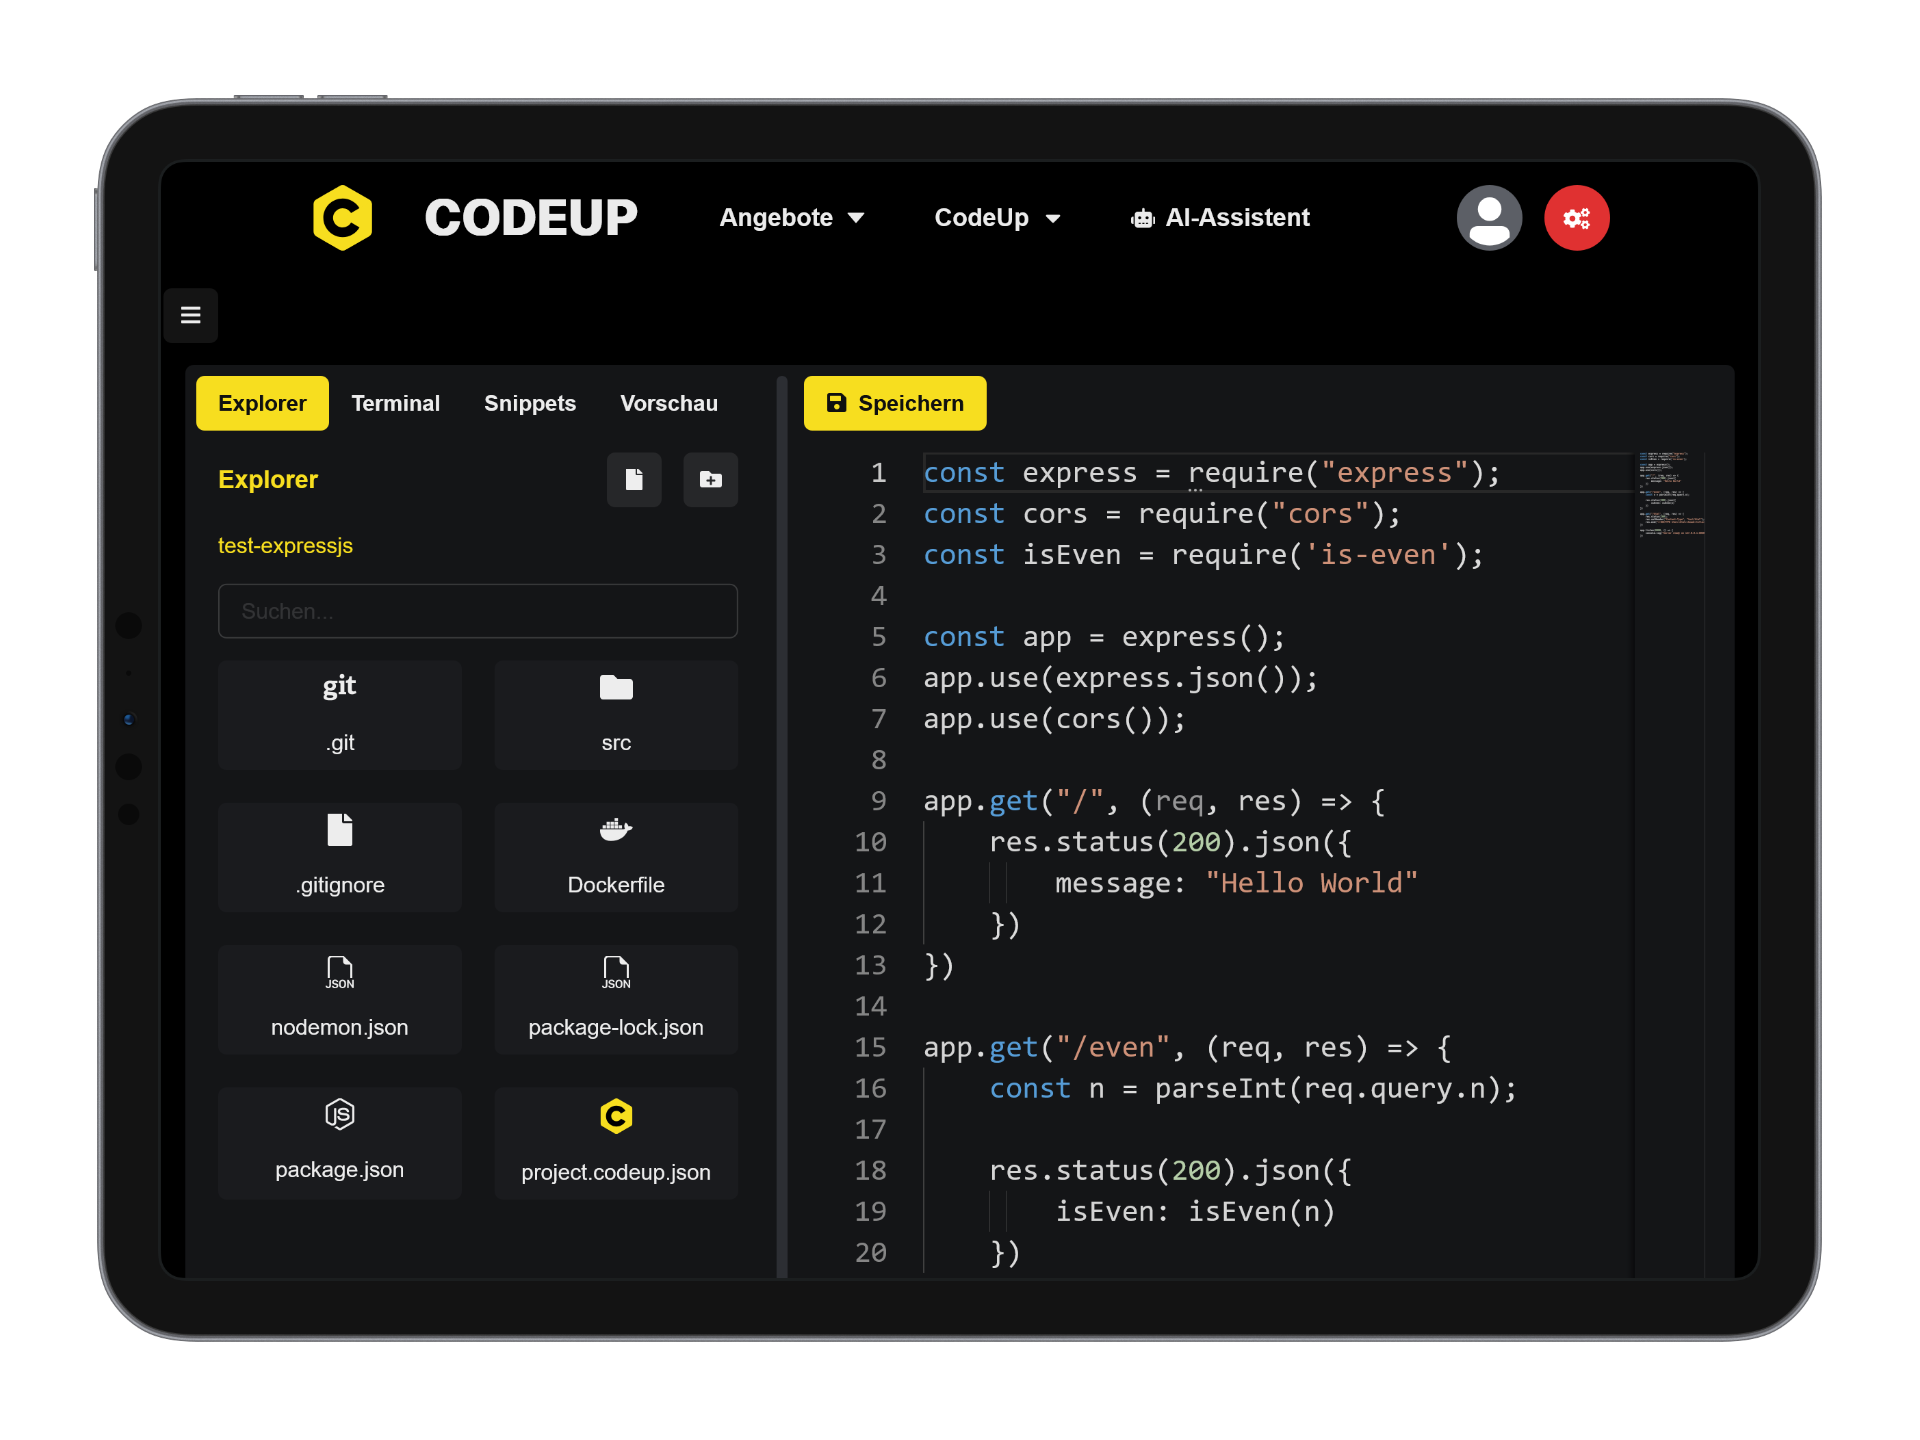
\includegraphics[width=0.6\textwidth]{assets/dev-suite}
        \caption{Dev-Suite}
        \label{fig:dev-suite}
    \end{figure}
    \subsubsection{CodeUp-Kids}
    Der CodeUp-Kids-Bereich ist speziell für jüngere Benutzer gedacht, die noch keine oder nur wenig Erfahrung im Programmieren haben.
    Hier gibt es eine einfache Programmierumgebung, die es dem Benutzer ermöglicht mit visuellen Blöcken zu programmieren.
    Diese Blöcke können miteinander verbunden werden, um einfache Webseiten zu erstellen.
    Das Block-System basiert auf der Blockly-Bibliothek\footnote{\bscite{blockly}}, die eine einfache und intuitive Programmierung ermöglicht.
    Blockly selbst ist aber nur für die grafische Darstellung zuständig, die dahinterliegende Programmiersprache ist InCode, eine eigens entwickelte Sprache, die für CodeUp angepasst wurde.
    InCode ist eine einfache Programmiersprache, die auf JavaScript basiert und es dem Benutzer ermöglicht, einfache Programme zu erstellen.
    Hierbei schreibt der Benutzer möglichst grammatikalisch korrekte Sätze, die dann in JavaScript-Code umgewandelt werden.
    So soll der Benutzer spielerisch an das Programmieren herangeführt werden und erste Erfahrungen sammeln.
    Weitere Informationen zu InCode sind im Anhang~\ref{sec:incodedoc} zu finden.
    \subsubsection{Code-Snippets}
    Code-Snippets (auch Code-Schnipsel genannt) kann der Benutzer selbst erstellen und verwalten.
    Diese Snippets können Code-Blöcke, Funktionen oder ganze Programme sein, die der Benutzer immer wieder verwenden möchte.
    Snippets können zusätzlich mit einer Sprache versehen werden, sodass der Benutzer leichter nach ihnen suchen kann und entsprechende Syntax-Hervorhebung bekommt.
    In jedem Editor, bis auf den CodeUp-Kids Bereich, gibt es eine Schaltfläche, die es dem Benutzer ermöglicht, ein Snippet einzufügen.
    So soll die Wiederverwendung von Code-Blöcken erleichtert werden und der Benutzer kann schneller und effizienter arbeiten.
    \subsubsection{Projektideen}
    Projektideen sind ein zentraler Bestandteil von CodeUp.
    Diese Ideen sollen den Benutzern Inspiration geben und ihnen helfen, eigene Projekte zu entwickeln.
    Jede Projektidee besteht aus einer Beschreibung, die das Projekt erklärt, und optional einer Demo, die das Projekt in Aktion zeigt.
    Bei vielen Ideen ist ebenfalls ein Link zu einem beispielhaften Quellcode enthalten, an dem sich der Benutzer orientieren kann.
\end{document}
